\section{Energy consumption} 
\label{sec:energy_consumption}
The energy consumptions has been measured for the sending mote.
Measurements are done by shunting the power supply to measure current draw.
Using an oscilloscope the current draw was integrated over time (See figures \ref{fig:UncompressedSend} and \ref{fig:CompressedSend}).
Then multiplying by the battery voltage yields energy consumption. \\
The measurements cover only the sending sequence, which consists of iterations of reading from flash, optional compression of the data, sending the packets and waiting for the acknowledgements. 

\textbf{NOTE:} The measurements on the oscilloscope are scaled by a factor of 10.
Hence the difference between what is shown in figures \ref{fig:UncompressedSend} / \ref{fig:CompressedSend} and equations \ref{eq:SendUncompressed} / \ref{eq:SendCompressed}.

\begin{equation}
E_{send} = 
\dfrac{\int_{}^{}V_{send}\ dt}
{R_{shunt}}
* V_{battery}
\end{equation}

\begin{equation}
R_{shunt} = 10\ \Omega
\qquad
V_{battery} = 2.734\ V
\end{equation}


\subsection{Uncompressed}

\begin{figure}[H]
\centering
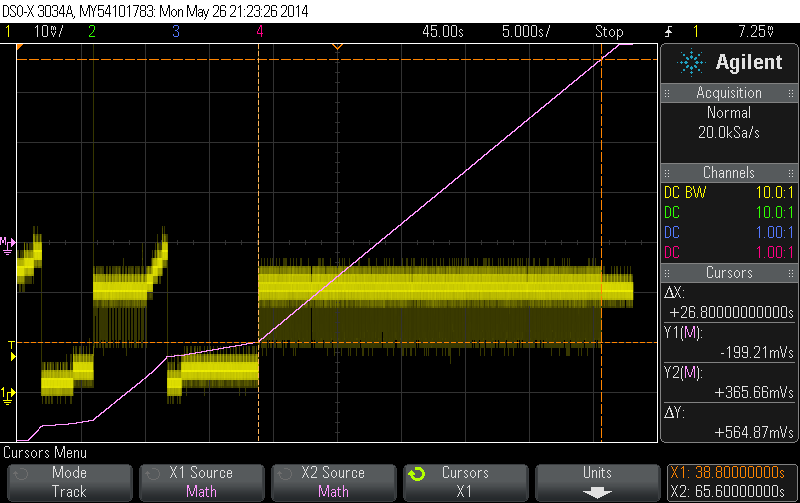
\includegraphics[width=0.8\linewidth]{UncompressedEnergy}
\caption{Voltage over $ 10\ \Omega $ current shunt during sending of an uncompressed image}
\label{fig:UncompressedSend}
\end{figure}

\begin{equation}
E_{send\ Uncompressed} = 
\dfrac{5.649\ Vs}
{10\ \Omega}
* 2.734\ V
=
1.544\ J
\label{eq:SendUncompressed}
\end{equation}

\subsection{Compressed}

\begin{figure}[H]
\centering
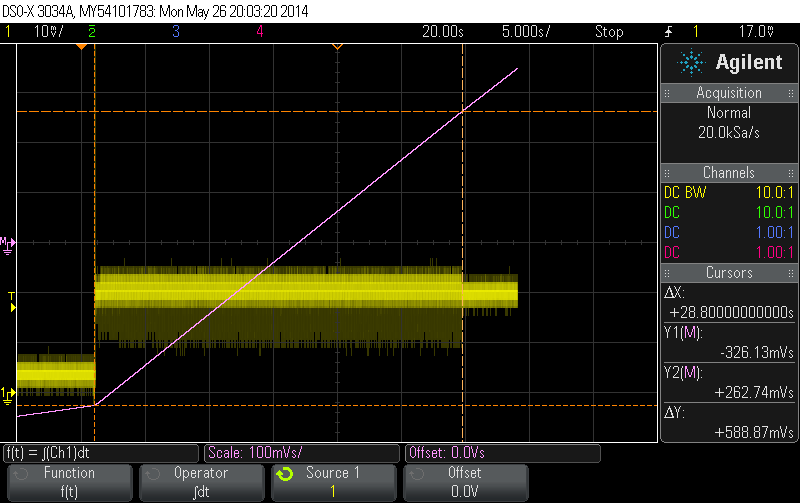
\includegraphics[width=0.8\linewidth]{CompressedEnergy}
\caption{Voltage over $ 10\ \Omega $ current shunt during sending of an compressed image}
\label{fig:CompressedSend}
\end{figure}

\begin{equation}
E_{send\ Uncompressed} = 
\dfrac{5.889\ Vs}
{10\ \Omega}
* 2.734\ V
=
1.601\ J
\label{eq:SendCompressed}
\end{equation}



